Let $\mathcal{H} = L^2 (0,1)$. We consider the stochastic Fisher-KPP 
    equation 
    \begin{equation}
        \label{eqn:fisher-kpp}
        \begin{aligned}
            d X(t, \xi) &= 
                \left[
                    \nu 
                    \partial_{\xi} ^ 2 X(t, \xi)
                    +
                    X(t, \xi) (1 -X(t, \xi) )
                \right]
                dt
                +
                dW(t, \xi),
            \\
            X(t, 0) &= X(t, 1) =0, \quad t>0, 
            \\
            X(0, \xi) & \in 
            \mathcal{H}, \ \xi \in [0, 1],
        \end{aligned}
    \end{equation}
    in the interval $[0, 1]$ and with initial function conditions
    $x(\xi):= $ and  $\widehat{x}(\xi) :=$.
    \todo{write the initial function conditions.}
    
    \paragraph{Experiment Description}
        We list in \Cref{tbl:parameters_fisher} the regarding parameters to
    obtain two solutions of stochastic Fisher equation with the conditions
    $x$ and $\widehat{x}$. \Cref{fig:fisher_kpp_approximation_t0} displays the 
    plots of this initial conditions. In \Cref{fig:likening_fisher_kpp} we 
    observe how the mentioned approximations remains close\textemdash blue
    color scale denotes the solution of equation \ref{eqn:fisher-kpp}
    with initial function condition $x(\xi)$, while yellow color corresponds 
    to the approximation with initial condition $\widehat{x}$. Since we employ
    transparency to obtain this 3D plot, the  purple scale results from the 
    closeness of the solutions. Further, \Cref{fig:errorfisher} suggest the 
    conclusion of \Cref{thm:ic_continuity}, that is, the solutions of equation
    \eqref{eqn:fisher-kpp} are continuous respect to initial conditions and 
    satisfies the estimation \eqref{s3.12}.

\begin{table}[H]
    \begin{tabular}{rc}
        \toprule
        $h$ 
        &
        $x$
        \\
        \bottomrule
    \end{tabular}
    \caption{}
    \label{tbl:parameters_fisher}
\end{table}

%
\begin{figure}[H]
    \centering
    \caption{
        Numerical Solution of the Fisher-KPP 
        \cref{eqn:fisher-kpp} 
        with initial conditions $x$, $y$ at time
        $t=0$.
     }
    \label{fig:fisher_kpp_approximation_t0}
    \includegraphics[width=\linewidth, keepaspectratio]%
    {StochasticFisherEquation/Approximation_t=0.eps}
\end{figure}
%
\begin{figure}[H]
    \centering
    \caption{
        Likening between two solution with closed 
        initial conditions $x$, $\widehat{x}$
        of the stochastic Fisher-KPP
        \cref{eqn:fisher-kpp}. See \cite{plotlyFisher}
        to obtain other camera perspectives.
     }
    \label{fig:likening_fisher_kpp}
    \includegraphics[width=\linewidth, keepaspectratio]%
    {StochasticFisherEquation/simulation_Approximation.png}
\end{figure}


\begin{figure}
    \centering
    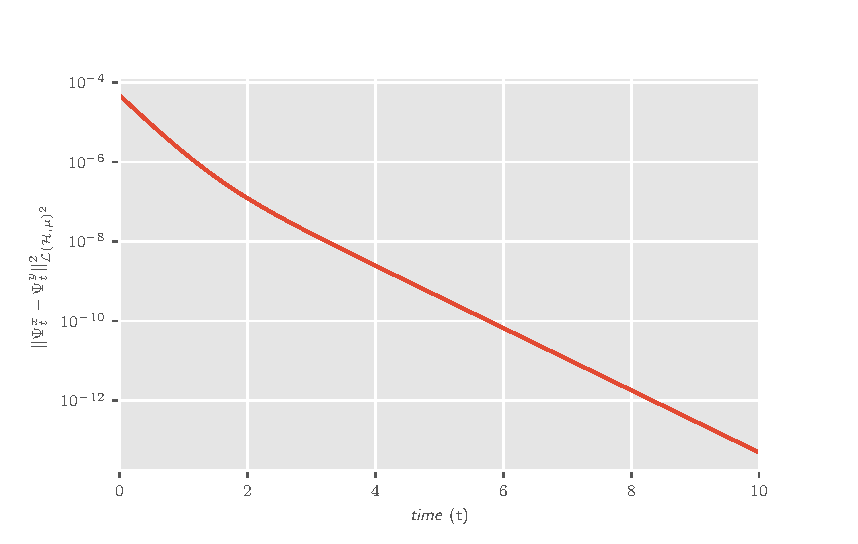
\includegraphics{StochasticFisherEquation/error_fisher}
     \caption{ $\mathcal{L}^2(\mathcal{H}, \mu)$
        distance between two solutions of the stochastic Fisher PDE 
        with initial conditions $x$, $\widehat{x}$.}
    \label{fig:errorfisher}
\end{figure}


\paragraph{Likening}
    In \Cref{fig:likening_fisher_kpp} we illustrate the distance between initial
    conditions distance between...
\todo{A paragraph to describe and stress the likening}
%
